\documentclass[11pt]{article}

\usepackage{amsmath, amssymb, amsthm} % ams packages %amsfonts is loaded by amssymb
% \usepackage[all,warning]{onlyamsmath}
\usepackage{graphics, graphicx} % graphics packages


\usepackage[margin=1in]{geometry} % more reasonable margins
\usepackage{booktabs} % prettier tables
\usepackage{units} % prettier fractions (?)

% Small sections of multiple columns
\usepackage{multicol}

\usepackage{bm}
\usepackage{float}
\usepackage{natbib}

\usepackage{tikz} % make graphics in latex
\usetikzlibrary{shapes,decorations}
\usetikzlibrary{arrows}
\usepackage{pgfplots} % to make plots in latex
\pgfplotsset{compat=newest} % compatibility issue
\usepackage{enumitem, comment}

% formatting
\usepackage{fancyhdr} % for changing headers and footers
\usepackage{url} % url 
\usepackage[normalem]{ulem}
\usepackage{color} % colored text + names %deprecated?



% hyperlink in the document
\usepackage{hyperref} % must be the last package loaded

\usepackage{comment}

\usepackage{parskip}

% notations
\newcommand{\one}{\ensuremath{\mathbf{1}}}
\newcommand{\zero}{\ensuremath{\mathbf{0}}}
\newcommand{\prob}{\ensuremath{\mathbf{P}}}
\newcommand{\expec}{\ensuremath{\mathbf{E}}}
\newcommand{\ind}{\ensuremath{\mathbf{I}}}
\newcommand{\reals}{\ensuremath{\mathbb{R}}}
\newcommand{\naturals}{\ensuremath{\mathbb{N}}}
\newcommand{\defeq}{\ensuremath{\triangleq}}
\newcommand{\sP}{\ensuremath{\mathsf{P}}}
\newcommand{\sQ}{\ensuremath{\mathsf{Q}}}
\newcommand{\sE}{\ensuremath{\mathsf{E}}}

\newcommand{\mbf}[1]{{\boldsymbol{\mathbf{#1}}}}
\renewcommand{\bm}{\mbf}


% environments
\newtheorem{theorem}{Theorem}

\newtheorem{proposition}{Proposition}
\newtheorem{corollary}{Corollary}
\newtheorem{lemma}{Lemma}
\newtheorem{remark}{Remark}
\newtheorem{definition}{Definition}
\newtheorem{assumption}{Assumption}


\title{\vspace{-20mm} Bayesian Machine Learning Midterm \\ \vspace{5mm}  \normalsize Instructor: Andrew Gordon Wilson}
\date{2020-10-29}
\author{\textbf{Guido Petri, netID gp1655} }
\newenvironment{solution}{\bigskip\noindent
                          \textbf{Solution}}

\begin{document}
\maketitle

\textbf{1. Radioactive particles}

\begin{enumerate}[label=\textbf{\alph*.}]
    \item Likelihood function.

        The likelihood function is simply the probability of the aggregate dataset. With $n, n_>, n_<$ representing indices (or lengths of these index sets) for which $x$ is in each set:

        $$
        p(\mathcal{D} | \lambda, a, b) = \prod_{i \in n} p(x_i)
        $$

        $$
        p(\mathcal{D} | \lambda, a, b) = \prod_{i \in n_<} p(x_i) \prod_{j \in n_>} p(x_j)
        $$

        $$
        p(\mathcal{D} | \lambda, a, b) = \prod_{i \in n_<} \lambda \exp (-\lambda x_i) \prod_{j \in n_>} \dfrac{1}{b - a}
        $$

        $$
        p(\mathcal{D} | \lambda, a, b) = \lambda^{n_<} \exp (-\lambda \sum_{i \in n_<} x_i) (\dfrac{1}{b - a})^{n_>}
        $$

        $$\square$$

    \item ML estimate for $\lambda$.

        Finding the ML estimate by taking the derivative of the likelihood with respect to $\lambda$ and setting it to $0$:

        $$
        \dfrac{\partial p(\mathcal{D} | \lambda, a, b)}{\partial \lambda} = \dfrac{\partial (\lambda^{n_<} \exp (-\lambda \sum_{i \in n_<} x_i) (\dfrac{1}{b - a})^{n_>})}{\partial \lambda} = 0
        $$

        Applying the product rule and the chain rule:

        $$
        0 = (\dfrac{1}{b - a})^{n_>} (\lambda^{n_< - 1} \exp (-\lambda \sum_{i \in n_<} x_i) (n_< - \lambda \sum_{i \in n_<} x_i))
        $$

        $$
        0 = (\dfrac{1}{b - a})^{n_>} \lambda^{n_< - 1} \exp (-\lambda \sum_{i \in n_<} x_i) (n_< - \lambda \sum_{i \in n_<} x_i)
        $$

        Solving for $\lambda$:

        $$
        0 = \exp (-\lambda \sum_{i \in n_<} x_i) (n_< - \lambda \sum_{i \in n_<} x_i)
        $$

        Since the exponential can never be $0$, then

        $$
        0 = n_< - \lambda \sum_{i \in n_<} x_i
        $$

        $$
        n_< = \lambda \sum_{i \in n_<} x_i
        $$

        $$
        \lambda  = \dfrac{n_<}{\sum_{i \in n_<} x_i}
        $$

        $$\square$$

    \item ML value for $b$ and its reasonability.

        Using the same process as for $\lambda$ above:

        $$
        \dfrac{\partial p(\mathcal{D} | \lambda, a, b)}{\partial b} = \dfrac{\partial (\lambda^{n_<} \exp (-\lambda \sum_{i \in n_<} x_i) (\dfrac{1}{b - a})^{n_>})}{\partial b} = 0
        $$

        $$
        \lambda^{n_<} \exp (-\lambda \sum_{i \in n_<} x_i) \dfrac{\partial ((\dfrac{1}{b - a})^{n_>})}{\partial b} = 0
        $$

        $$
        \dfrac{\partial ((\dfrac{1}{b - a})^{n_>})}{\partial b} = 0
        $$

        $$
        - n_> (\dfrac{1}{b - a})^{n_> + 1} = 0
        $$

        $$
        (\dfrac{1}{b - a})^{n_> + 1} = 0
        $$

        Here we see that the term on the left will never actually achieve $0$, but it can be approximated in the limit:

        $$
        \lim_{b \rightarrow \infty} (\dfrac{1}{b - a})^{n_> + 1} = 0
        $$

        Thus the maximum likelihood value for $b$ is actually $\infty$. This is not a reasonable estimate for $b$, of course, since that would imply that our window $[a,b]$ is actually of infinite size, and that any value beyond $a$ is possible. This makes our uniform probability distribution across $[a,b]$ degenerate, since the value of the distribution at any point is $0$.

    \item Prior for $p(\lambda)$, posterior $p(\lambda|\mathcal{D})$, predictive distribution $p(x|\mathcal{D})$. Graphical model for joint distribution.

        I think a reasonable prior for $\lambda$ would be a uniform across the space $[0, a]$. We don't know much about the parameter, so I would place a uniform distribution on it. To find the borders of the probability distribution, we must examine the little we do know. The $\lambda$ parameter should be, at the very least, positive; this means that the uniform distribution should start at $0$. Since we observe $n_<$ values in $[0, a]$, I would also assume that the rate parameter is something less than $a$, since otherwise this would be an extremely improbable dataset. This is supported by the mean of the exponential distribution with $\lambda = a$: it would be $\frac{1}{a}$, i.e. we would expect to see one sample in $[0, a]$ if our $\lambda$ was $a$. Thus, the uniform is bounded by $0$ and $a$, and the prior probability for any specific value of $\lambda$ is $\frac{1}{a}$.

        The posterior $p(\lambda|\mathcal{D})$ can be written as a function of the likelihood, prior and marginal likelihood:

        $$
        p(\lambda|\mathcal{D}) = \dfrac{p(\lambda) p(\mathcal{D}|\lambda)}{p(\mathcal{D})}
        $$

        where $p(\lambda)$ is the aforementioned prior, $p(\mathcal{D}|\lambda)$ is the likelihood, and $p(\mathcal{D})$ is the marginal likelihood.

        To compute the posterior predictive distribution $p(x|\mathcal{D})$, we must take the probability distribution for a given $\lambda$ and integrate across all possible values of $\lambda$:

        $$
        p(x|\mathcal{D}) = \int p(x|\lambda, \mathcal{D}) p(\lambda|\mathcal{D}) d \lambda
        $$

        $$
        p(x|\mathcal{D}) = \int \lambda \exp(-\lambda x) \dfrac{p(\lambda) p(\mathcal{D}|\lambda)}{p(\mathcal{D})} d \lambda
        $$

        $$
        p(x|\mathcal{D}) = \dfrac{1}{a \cdot p(\mathcal{D})} \int \lambda \exp(-\lambda x) p(\mathcal{D}|\lambda) d \lambda
        $$

        Using the likelihood from (a) above:

        $$
        p(x|\mathcal{D}) = \dfrac{1}{a \cdot p(\mathcal{D})} \int \lambda \exp(-\lambda x) \lambda^{n_<} \exp (-\lambda \sum_{i \in n_<} x_i) (\dfrac{1}{b - a})^{n_>} d \lambda
        $$

        $$
        p(x|\mathcal{D}) = (\dfrac{1}{b - a})^{n_>} \dfrac{1}{a \cdot p(\mathcal{D})} \int \exp(-\lambda x) \lambda^{n_< + 1} \exp (-\lambda \sum_{i \in n_<} x_i) d \lambda
        $$

        $$
        p(x|\mathcal{D}) = (\dfrac{1}{b - a})^{n_>} \dfrac{1}{a \cdot p(\mathcal{D})} \int \lambda^{n_< + 1} \exp (-\lambda (x + \sum_{i \in n_<} x_i)) d \lambda
        $$

        With the upper incomplete gamma function and $c = (x + \sum_{i \in n_<} x_i)$, and using the integral limits of $[0, a]$:

        $$
        p(x|\mathcal{D}) = (\dfrac{1}{b - a})^{n_>} \dfrac{1}{a \cdot p(\mathcal{D})} (\dfrac{a^{n_< + 1} (c a)^{- n_< - 1} \Gamma(n_< + 2, c a)}{c} - \dfrac{0^{n_< + 1} (c 0)^{- n_< - 1} \Gamma(n_< + 2, c 0)}{c})
        $$

        $$
        p(x|\mathcal{D}) = (\dfrac{1}{b - a})^{n_>} \dfrac{1}{a \cdot p(\mathcal{D})} \dfrac{a^{n_< + 1} (c a)^{- n_< - 1} \Gamma(n_< + 2, c a)}{c}
        $$

        The graphical model for this probability distribution is:

        \begin{figure}[H]
            \centering
            \includegraphics[scale=0.45]{midterm_dgm.pdf}
            \caption{Joint distribution over all parameters of the model in exercise 1.}
        \end{figure}

    \item Evaluation of the marginal likelihood via Simple Monte Carlo.

        We can evaluate the marginal likelihood $p(\mathcal{D}$ by drawing samples from the prior $p(\lambda)$ and then evaluating $p(\mathcal{D}|\lambda_{draw})$. The marginal likelihood is then found by the sum of these likelihoods, weighed by the probability of the specific value of $\lambda$. Since my prior is a uniform over $[0, a]$, this is simply

        $$
        \dfrac{\sum_{j \in draws} p(\mathcal{D}|\lambda_{j})}{a}
        $$

        This is a reasonable estimate of the marginal likelihood for enough draws, but not a very good estimate for a very low number of draws. This is because the Monte Carlo simulation method only asymptotically approximates the true probability distribution that we try to approximate, via the law of large numbers.

\end{enumerate}

\textbf{2. Genes}

\begin{enumerate}[label=\textbf{\alph*.}]

    \item Likelihood of the data $p(\bm{y} | \bm{w}, \alpha, \lambda, X)$.

        Let's start by describing the model further:

        $$
        p(z=1|\bm{x}, \bm{w}) = \sigma(\bm{w}^T \bm{x})
        $$

        $$
        p(z=0|\bm{x}, \bm{w}) = 1 - \sigma(\bm{w}^T \bm{x})
        $$

        $$
        p(y=1|z=1) = \alpha
        $$

        $$
        p(y=0|z=1) = 1 - \alpha
        $$

        $$
        p(y=0|z=0) = \lambda
        $$

        $$
        p(y=1|z=0) = 1 - \lambda
        $$

        Thus, for a given $\bm{x}$, we can marginalize the latent variable $z$ out:

        $$
        p(y|\bm{x}, \bm{w}) = \sum_{z \in \{0, 1\}} p(y|z) p(z|\bm{x}, \bm{w})
        $$

        $$
        p(y|\bm{x}, \bm{w}) = p(y|z=1) p(z=1|\bm{x}, \bm{w}) + p(y|z=0) p(z=0|\bm{x}, \bm{w})
        $$

        For $y=1$:

        $$
        p(y=1|\bm{x}, \bm{w}) = \alpha \sigma(\bm{w}^T \bm{x}) + (1 - \lambda) (1 - \sigma(\bm{w}^T \bm{x}))
        $$

        For $y=0$:

        $$
        p(y=0|\bm{x}, \bm{w}) = (1 - \alpha) \sigma(\bm{w}^T \bm{x}) + \lambda (1 - \sigma(\bm{w}^T \bm{x}))
        $$

        The likelihood for the entire dataset is just the aggregate multiplied probability of each datapoint:

        $$
        p(\bm{y}|\bm{w}, \alpha, \lambda, X) = \prod_{i=1}^n p(y_i|\bm{w}, \alpha, \lambda, x_i)
        $$

        With $\theta$ being the count of $y=1$ (and, correspondingly, $n - \theta$ being the count of $y=0$):

        $$
        p(\bm{y}|\bm{w}, \alpha, \lambda, X) = (\alpha \sigma(\bm{w}^T X) + (1 - \lambda) (1 - \sigma(\bm{w}^T X)))^{\theta} ((1 - \alpha) \sigma(\bm{w}^T X) + \lambda (1 - \sigma(\bm{w}^T X)))^{n - \theta}
        $$

    \item Priors for $\alpha, \lambda$ and the directed graphical model.

        Since this is a "binary classification" kind of problem, where only two classes exist, we can use a Beta distribution prior:

        $$
        B = \Gamma(c+d) \dfrac{\alpha^{c-1} (1 - \alpha)^{d-1}}{\Gamma(c)\Gamma(d)}
        $$

        (or correspondingly, for $\lambda$):

        $$
        B = \Gamma(e+f) \dfrac{\lambda^{e-1} (1 - \lambda)^{f-1}}{\Gamma(e)\Gamma(f)}
        $$

        Since our domain expertise indicates that $y$ has mostly the same values as $z$, then we can place strong priors that are skewed towards $1$ on both $\alpha$ and $\lambda$. This means that $c << d$ and $e << f$. Assuming that $\gamma^2$ is not random, the resulting directed graphical model is:

        \begin{figure}[H]
            \centering
            \includegraphics[scale=0.45]{midterm_dgm_2.pdf}
            \caption{Joint distribution over all parameters of the model in exercise 2.}
        \end{figure}

    \item Predictive distribution $p(y_*|x_*, \mathcal{D}, \bm{v})$, Simple Monte Carlo estimation, and over/underconfidence.

        The predictive distribution $p(y_*|x_*, \mathcal{D}, \bm{v})$ is:

        $$
        p(y_*|x_*, \mathcal{D}, \bm{v}) = \int p(y_*|x_*, \bm{w}, \mathcal{D}, \bm{v}) p(\bm{w}|\mathcal{D}, \bm{v}) d\bm{w}
        $$

        The posterior for $\bm{w}$ is

        $$
        p(\bm{w}|\mathcal{D}, \bm{v}) = \dfrac{p(\bm{w}|\bm{v}) p(\mathcal{D}|\bm{w}, \bm{v})}{p(\mathcal{D}| \bm{v})}
        $$

        Plugging this in:

        $$
        p(y_*|x_*, \mathcal{D}, \bm{v}) = \int p(y_*|x_*, \bm{w}, \mathcal{D}, \bm{v}) \dfrac{p(\bm{w}|\bm{v}) p(\mathcal{D}|\bm{w}, \bm{v})}{p(\mathcal{D}| \bm{v})} d\bm{w}
        $$

        $$
        p(y_*|x_*, \mathcal{D}, \bm{v}) = \dfrac{1}{p(\mathcal{D}| \bm{v})} \int p(y_*|x_*, \bm{w}, \mathcal{D}, \bm{v}) p(\bm{w}|\bm{v}) p(\mathcal{D}|\bm{w}, \bm{v}) d\bm{w}
        $$

        $$
        p(y_*|x_*, \mathcal{D}, \bm{v}) = \dfrac{1}{p(\mathcal{D}| \bm{v})} \int \mathcal{N}(\bm{w}|0, \gamma^2 \ind) * $$$$ (\alpha \sigma(\bm{w}^T X) + (1 - \lambda) (1 - \sigma(\bm{w}^T X)))^{\theta + 1} ((1 - \alpha) \sigma(\bm{w}^T X) + \lambda (1 - \sigma(\bm{w}^T X)))^{n - \theta} d\bm{w}
        $$

        (line broken otherwise it would not fit on page)

        This integral can be estimated with Simple Monte Carlo by drawing samples from the distribution of $\bm{w}$ and calculating the above probabilities, then weighing by the probability of having achieved that specific value of $\bm{w}$.

        This model is likely overconfident, since we are assuming $\alpha$ and $\lambda$ are close to $1$. This means that our probabilities end up being multiplied by values close to $0$ or $1$, so they do not change much; whereas if we had the product of several values close to $0.5$, we would have underconfidence.

    \item Posterior, MCMC method for sampling.

        The posterior is

        $$
        p(\bm{w}, \alpha, \lambda|\bm{y},\bm{v}) = \dfrac{p(\bm{w}, \alpha, \lambda|\bm{v}) p(\bm{y}|\bm{w}, \alpha, \lambda, \bm{v})}{p(\bm{y}|\bm{v})}
        $$

        With the priors from exercise (b) and the likelihood $\mathcal{L}$ from (a):

        $$
        p(\bm{w}, \alpha, \lambda|\bm{y},\bm{v}) = \dfrac{p(\bm{w}|\gamma^2) p(\alpha|c,d) p(\lambda|e,f) \mathcal{L}(y)}{p(\bm{y}|\bm{v})}
        $$

        (summarized since otherwise it would not fit on the page:)

        $$
        p(\bm{w}|\gamma^2) = \mathcal{N}(0, \gamma^2 \ind)
        $$

        $$
        p(\alpha|c,d) = \Gamma(c+d) \dfrac{\alpha^{c-1} (1 - \alpha)^{d-1}}{\Gamma(c)\Gamma(d)}
        $$

        $$
        p(\lambda|e,f) = \Gamma(e+f) \dfrac{\lambda^{e-1} (1 - \lambda)^{f-1}}{\Gamma(e)\Gamma(f)}
        $$

        Here I assumed that $\bm{w}, \alpha, \lambda$ are all independent and thus factorize into their individual probability distributions. I also assumed that there were no dependences on other hyperparameters (e.g. $\alpha$ is independent from $e, f$).

        To sample from this posterior, I could use slice sampling, since I can evaluate this posterior up to a constant and the posterior is unimodal (since there is only one normal distribution and two beta distributions for priors). This also means that I do not need to do any tuning of this posterior in order to get a good approximation.

\end{enumerate}

\textbf{3. Bayesian approaches}

\begin{enumerate}[label=\textbf{\alph*.}]

    \item Expressivity of a model dependent on data amount: true/false.

        \textit{True}: In a frequentist perspective, if we use a model that is too flexible for a low number of datapoints, we run the risk of "overfitting" and not being able to generalize to outside of the training set. That is, the model would learn to fit not only the underlying trend, but also the noise inherent to the training data. As a result, we're forced to use less flexible models in order to be able to generalize to unseen data (by only fitting the underlying trend, not the noise).

        \textit{False}: However, using less flexible models doesn't actually correspond to our beliefs about the system. Most phenomena that we try to model using machine learning/statistical methods are complex and have several moving parts and dependencies, meaning there is indeed a lot of complexity in the data. Not only that, and perhaps more importantly, the complexity of the data-generating distribution doesn't change depending on the number of observed datapoints! So we shouldn't use less flexible models for the situation with fewer data points - we should use the same model for both $40000$ datapoints and $10$ datapoints, and this model should be very flexible in order to capture as much information as possible.

    \item Bayesian vs Frequentist approaches.

        Bayesian methods make very different predictions to ML approaches, even for uniform (or uninformative) priors, especially when the number of datapoints is small. For instance, if we were to flip a coin once, and it came up heads, the maximum likelihood approach would set $p(heads)=1$, whereas the Bayesian approach with a uniform prior would set $p(heads)$ as a distribution of possible values, each with a different "confidence". Taking the probability that is highest (aka the MAP) would yield the same value as the ML approach, but the Bayesian would recognize that there are also other possibilities for the coin's bias/fairness. In this example, the Bayesian would not guess with certainty ($p=1$) that the next coin flip is heads, but would assign a higher probability to it.

        For more complex models, and different priors, we will use the following image, sourced from the paper \textit{Bayesian Deep Learning and a Probabilistic Perspective of Generalization}, by Andrew Gordon Wilson and Pavel Izmailov:

        \begin{figure}[H]
            \centering
            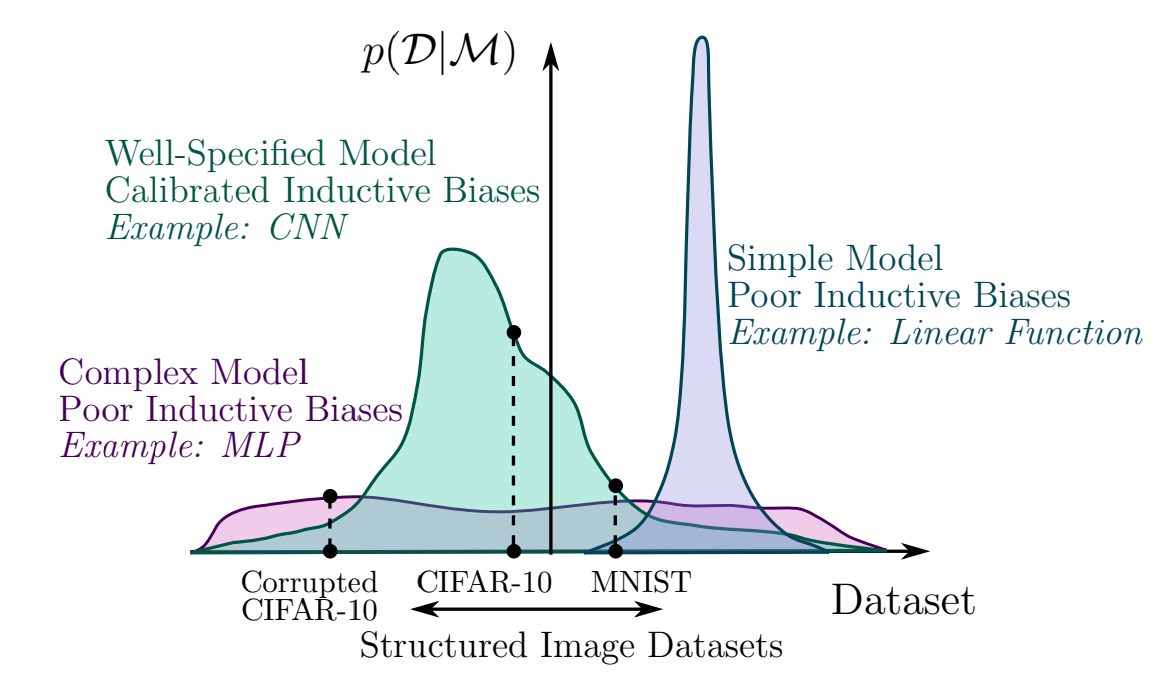
\includegraphics[scale=0.45]{midterm_mll.png}
            \caption{Different models and the probability they assign to a dataset $\mathcal{D}$. Source: https://arxiv.org/pdf/2002.08791.pdf}
        \end{figure}

        In the above image, we can see that different models have different priors and can describe datasets with different probabilities. For instance, the MLP can describe many datasets, but places a low probability on any given dataset, while the linear function can describe fewer datasets but assigns much higher probability to a given dataset. If we imagine the same phenomenon, but with a uniform prior, we would still have much higher probability on a per-dataset basis for the linear function than for the MLP. This means that, even though the MLP might be able to describe the data perfectly (with maximum likelihood), the Bayesian approach could argue for the simple model because its marginal likelihood is far higher.

        Asymptotically, both the frequentist and the uninformative-prior-Bayesian approaches should arrive at the same solution. However, this requires an infinite amount of data, which we do not have access to.

    \item KL divergence and approximating the posterior with Laplace, VI, EP.

        Illustrating the different distributions achieved through the estimation procedures:

        \begin{figure}[H]
            \centering
            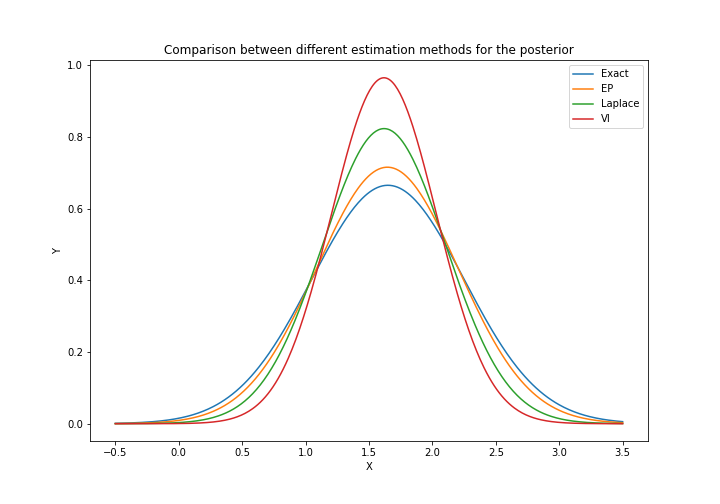
\includegraphics[scale=0.45]{midterm_posterior_estimation.png}
            \caption{Comparison between different estimation methods for the posterior.}
        \end{figure}

        As we can see from the image above, different methods of estimating the posterior have different "accuracies" in how close they can actually estimate the distribution in question. EP is the best method, followed by the Laplace approximation and then by VI.

        The \textit{Expectation Propagation} (EP) method minimizes the KL divergence from the true distribution $p$ to the approximate distribution $q$ by changing $q$. This method approximates the posterior very well because it tries to create a reference that is very close to the posterior, rather than take the posterior as a reference distribution. As we can see from the results, it also has the best approximation in this case.

        The Laplace method for estimating the posterior involves several approximations, and thus is not very accurate. One of the big inaccuracies in it stems from the Taylor expansion of the logarithm of the proposal distribution only to the second term, and not to further terms. This leads to slightly inaccurate estimation of the peak of the Gaussian and its variance, but since this is in log-space, the inaccuracy gets inflated in "real" space. This can be seen in Table 1: the estimated posterior mean is relatively far from the true mean, and the estimated variance is much further than EP.

        Finally, VI estimates the posterior by trying to approximate its moments (mean and variance, in this case), as measured by minimizing the KL divergence $KL(q||p)$. Since this is a Gaussian, we should expect this to approximate the posterior very well; but because it is minimizing the KL divergence measured from $q$ to $p$, it does not perform very well.

    \item Different Laplace approximation.

        Visualizing the new Laplace approximation:

        \begin{figure}[H]
            \centering
            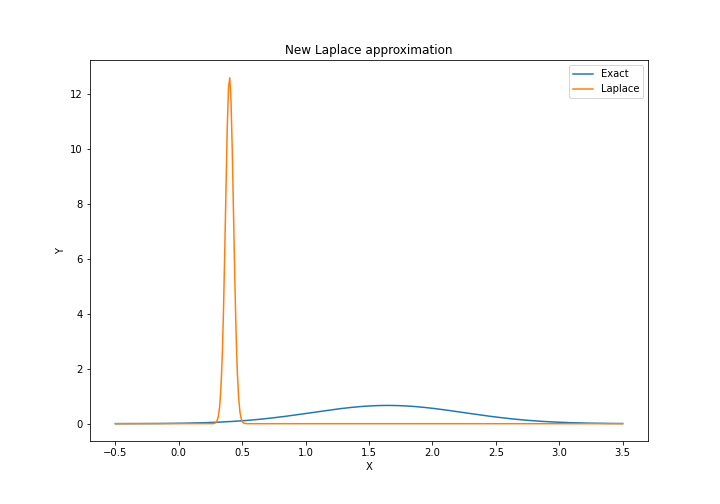
\includegraphics[scale=0.45]{midterm_laplace.png}
            \caption{New Laplace approximation compared to exact posterior.}
        \end{figure}

        What might have happened in this case is that we chose the incorrect MAP for estimating the posterior with Laplace. If we choose an incorrect MAP - in this case, it was likely a set of outliers - then we suffer from something like a "mode collapse" in which the estimated posterior mean is far from the true mean, and the estimated variance is much smaller than the truth. This can be seen in the image above.

\end{enumerate}

\textbf{4. Gaussian Processes}

\begin{enumerate}[label=\textbf{\alph*.}]
    
    \item $g(\bm{x})|a(\bm{x})$ is/isn't a GP.

        It is a Gaussian process. For a given value of $a(\bm{x})$, the term $g(\bm{x})|a(\bm{x})$ "collapses" to simply $c \cdot y(\bm{x})$, with $c$ as a constant. This is a GP if $y(\bm{x})$ is a GP, since a scaling factor does not change whether a term is a GP or not. $y(\bm{x})$ is also a GP, since adding a normal distribution to a GP (in  this case, $f(\bm{x})$) also keeps the term as a GP. Thus:

        $f(\bm{x})$ is GP $\rightarrow$ $f(\bm{x}) + \epsilon (\bm{x})$ is GP $\rightarrow$ $y(\bm{x})$ is GP $\rightarrow$ $g(\bm{x})|a(\bm{x})$ is GP.

    \item Mean/covariance function of $g(\bm{x})|a(\bm{x})$.

        The mean of the GP is $0$, the same as the mean of $f(\bm{x})$, since we only did two operations: addition of normally-distributed noise (does not affect the mean) and scaling (affects the mean, but any constant times $0$ is $0$).

        The covariance function $K$ of the GP is simply changing the kernel $k$ with the element-wise addition of $\sigma^2$ and the scaling by $a(\bm{x})$:

        $$
        K = a(\bm{x})(k + \sigma^2)
        $$

    \item Marginalized $a(\bm{x})$, $g(\bm{x})$ is/isn't a GP.

        If we marginalize $a(\bm{x}) = w^T \phi(\bm{x})$ out of $g(\bm{x})$, then we still have a GP. This is because we are marginalizing over an entire multivariate normal distribution; the remainder of $g(\bm{x})$ is dependent on $f(\bm{x})$ which is still a GP.

    \item Difference between two GP models $g(\bm{x})$ and $h(\bm{x})$.

        The difference between the two models stems from the difference in how they model noise. $g(\bm{x})$ models noise as a single parameter that is "shared" across all dimensions, whereas $h(\bm{x})$ has a different amount of noise in each dimension. This is equivalent to the difference between the RBF and the ARD kernels.

        Since $g(\bm{x})$ has more constraints on the "amount of noise" it allows on the dataset (because it must be the same across all dimensions), it manages to extract more structure out of the data.

\end{enumerate}

\end{document}
